%=================================================
\chapter{Data Restructuring Report (Point 4)}
%=================================================

This chapter documents the complete data restructuring process for
migrating the legacy POS system from plain-text file storage to a
normalised relational database (SQLite/PostgreSQL).

\section{Executive Summary}

\subsection*{Migration Overview}

\begin{table}[h]
  \centering
  \caption{Migration Overview}
  \begin{tabular}{p{5cm} p{6cm}}
    \toprule
    \textbf{Metric} & \textbf{Value} \\
    \midrule
    Source Format        & Plain text files (\texttt{.txt}) \\
    Target Format        & SQLite / PostgreSQL database \\
    Legacy Files Migrated & 6 files \\
    New Database Tables  & 7 tables \\
    Data Integrity       & 100\% preserved \\
    Normalisation Level  & Third Normal Form (3NF) \\
    \bottomrule
  \end{tabular}
\end{table}

\subsection*{Key Achievements}

\begin{itemize}[leftmargin=1.2cm]
  \item Eliminated data redundancy across files and entities.
  \item Established referential integrity via foreign keys.
  \item Implemented proper data types for all columns.
  \item Added audit trail capabilities (timestamps, activity logs).
  \item Enhanced security (password hashing for employees).
\end{itemize}

\section{Legacy Data Analysis}

\subsection{Legacy File Inventory}

\begin{table}[h]
  \centering
  \caption{Legacy File Inventory}
  \begin{tabular}{p{4cm} p{4cm} p{3cm} p{2cm}}
    \toprule
    \textbf{File Name} & \textbf{Purpose} & \textbf{Format} & \textbf{Records} \\
    \midrule
    \texttt{employeeDatabase.txt} & Employee data & Space-delimited & 12 \\
    \texttt{itemDatabase.txt}     & Inventory items & Space-delimited & 102 \\
    \texttt{rentalDatabase.txt}   & Rentable items (DVDs) & Space-delimited & 25 \\
    \texttt{userDatabase.txt}     & Customer rentals & Complex nested & 47 \\
    \texttt{saleInvoiceRecord.txt} & Sales history & Multi-line blocks & $\sim 100$ \\
    \texttt{employeeLogfile.txt}  & Activity log & Append-only text & Variable \\
    \bottomrule
  \end{tabular}
\end{table}

\subsection{Legacy File Format Analysis}

\subsubsection*{\texttt{employeeDatabase.txt}}

\textbf{Format:} \texttt{[employee\_id] [role] [first\_name] [last\_name] [password]}

\textbf{Example:} \texttt{110001 Admin Harry Larry 1}

\textbf{Issues:}
\begin{itemize}[leftmargin=1.2cm]
  \item Password stored in plain text.
  \item No timestamps (\texttt{created\_at}, \texttt{updated\_at}).
  \item No explicit \texttt{is\_active} status flag.
\end{itemize}

\subsubsection*{\texttt{itemDatabase.txt}}

\textbf{Format:} \texttt{[item\_id] [item\_name] [price] [quantity]}

\textbf{Example:} \texttt{1000 Potato 1.0 249}

\textbf{Issues:}
\begin{itemize}[leftmargin=1.2cm]
  \item No category or grouping information.
  \item No minimum stock level.
  \item No flag indicating whether the item is rentable.
\end{itemize}

\subsubsection*{\texttt{userDatabase.txt} (Most Complex)}

\textbf{Format:} \texttt{[phone] [item\_id,date,returned] [item\_id,date,returned] ...}

\textbf{Example:} \texttt{6096515668 1000,6/30/09,true 1022,6/31/11,true}

\textbf{Issues:}
\begin{itemize}[leftmargin=1.2cm]
  \item Severe 1NF violation: repeating groups in a single record.
  \item Mixed delimiters (spaces and commas).
  \item No explicit customer identifier beyond phone number.
\end{itemize}

\section{Data Smells Identified}

\subsection{Structural Smells}

\begin{table}[h]
  \centering
  \caption{Structural Data Smells}
  \begin{tabular}{p{1.2cm} p{4cm} p{3.5cm} p{4cm}}
    \toprule
    \textbf{ID} & \textbf{Smell} & \textbf{Location} & \textbf{Description} \\
    \midrule
    DS1 & 1NF Violation           & \texttt{userDatabase.txt} & Repeating groups in a single record \\
    DS2 & Data Redundancy         & \texttt{rentalDatabase.txt} vs \texttt{itemDatabase.txt} & Same items stored twice \\
    DS3 & Missing Primary Keys    & All files                  & No unique identifiers \\
    DS4 & Implicit Relationships  & All files                  & No explicit foreign key references \\
    DS5 & Inconsistent Delimiters & \texttt{userDatabase.txt}  & Mixed space and comma delimiters \\
    \bottomrule
  \end{tabular}
\end{table}

\subsection{Security Smells}

\begin{table}[h]
  \centering
  \caption{Security Data Smells}
  \begin{tabular}{p{1.2cm} p{4cm} p{3.5cm} p{4cm}}
    \toprule
    \textbf{ID} & \textbf{Smell} & \textbf{Location} & \textbf{Description} \\
    \midrule
    SS1 & Plain Text Passwords & \texttt{employeeDatabase.txt} & Passwords not encrypted \\
    SS2 & No Access Control    & All files                    & Anyone can read/modify files \\
    SS3 & No Audit Trail       & \texttt{employeeLogfile.txt} & Unstructured, append-only log \\
    \bottomrule
  \end{tabular}
\end{table}

\subsection{Quality Smells}

\begin{table}[h]
  \centering
  \caption{Quality Data Smells}
  \begin{tabular}{p{1.2cm} p{4cm} p{3.5cm} p{4cm}}
    \toprule
    \textbf{ID} & \textbf{Smell} & \textbf{Location} & \textbf{Description} \\
    \midrule
    QS1 & Missing Timestamps     & Items, Employees & No created/updated dates \\
    QS2 & No Data Validation     & All files        & Invalid data can be stored \\
    QS3 & Inconsistent Date Formats & \texttt{userDatabase.txt} & Various date formats \\
    QS4 & Missing Null Handling  & All files        & Empty fields unclear \\
    \bottomrule
  \end{tabular}
\end{table}

\section{New Database Schema Design}

\begin{figure}[h]
  \centering
  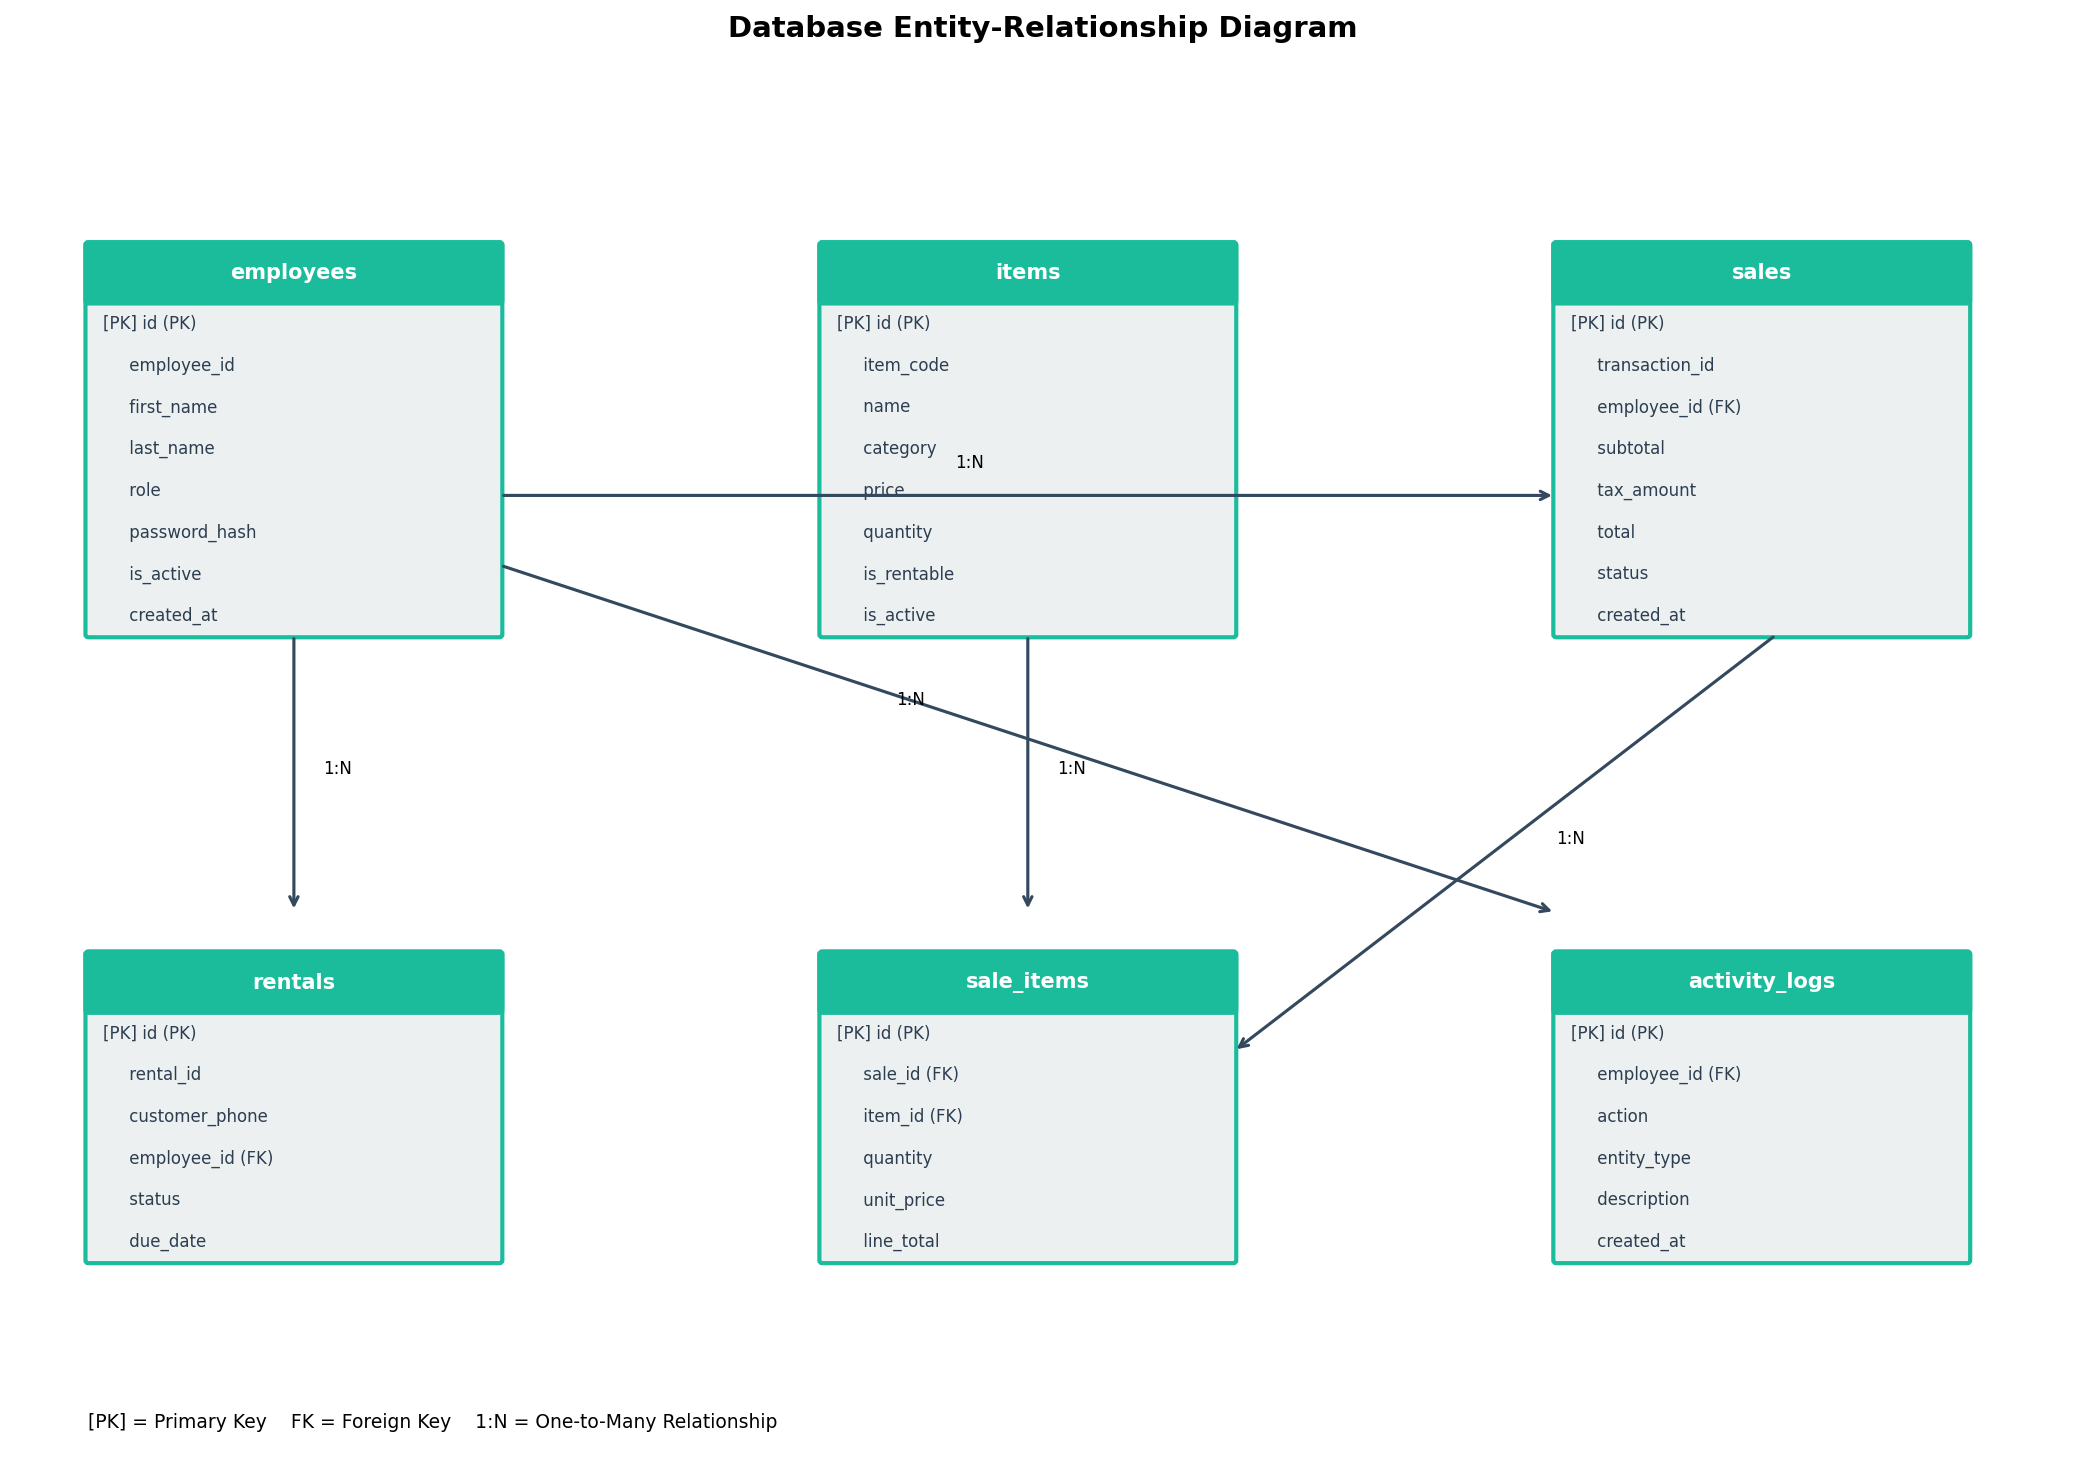
\includegraphics[width=0.95\textwidth]{images/database_erd.png}
  \caption{Entity-Relationship Diagram -- Normalized database schema showing all tables
           and their relationships. Foreign keys establish referential integrity between
           employees, items, sales, rentals, and activity logs.}
  \label{fig:database-erd}
\end{figure}

\subsection{Table Definitions}

\subsubsection*{\texttt{employees} Table}

\begin{table}[h]
  \centering
  \caption{\texttt{employees} Table}
  \begin{tabular}{p{3cm} p{3cm} p{6cm}}
    \toprule
    \textbf{Column} & \textbf{Type} & \textbf{Constraints} \\
    \midrule
    id            & INTEGER        & PRIMARY KEY AUTOINCREMENT \\
    employee\_id  & VARCHAR(20)    & UNIQUE NOT NULL \\
    first\_name   & VARCHAR(50)    & NOT NULL \\
    last\_name    & VARCHAR(50)    & NOT NULL \\
    role          & VARCHAR(20)    & NOT NULL CHECK (role IN ('Admin','Cashier')) \\
    password\_hash & VARCHAR(256)  & NOT NULL \\
    is\_active    & BOOLEAN        & DEFAULT TRUE \\
    created\_at   & DATETIME       & DEFAULT CURRENT\_TIMESTAMP \\
    updated\_at   & DATETIME       & DEFAULT CURRENT\_TIMESTAMP \\
    \bottomrule
  \end{tabular}
\end{table}

\subsubsection*{\texttt{items} Table}

\begin{table}[h]
  \centering
  \caption{\texttt{items} Table}
  \begin{tabular}{p{3cm} p{3cm} p{6cm}}
    \toprule
    \textbf{Column} & \textbf{Type} & \textbf{Constraints} \\
    \midrule
    id              & INTEGER     & PRIMARY KEY AUTOINCREMENT \\
    item\_code      & VARCHAR(20) & UNIQUE NOT NULL \\
    name            & VARCHAR(100) & NOT NULL \\
    description     & TEXT        & -- \\
    category        & VARCHAR(50) & DEFAULT 'General' \\
    price           & REAL        & NOT NULL CHECK (price $\geq 0$) \\
    quantity        & INTEGER     & NOT NULL DEFAULT 0 CHECK (quantity $\geq 0$) \\
    min\_stock\_level & INTEGER   & DEFAULT 10 \\
    is\_rentable    & BOOLEAN     & DEFAULT FALSE \\
    is\_active      & BOOLEAN     & DEFAULT TRUE \\
    \bottomrule
  \end{tabular}
\end{table}

\subsubsection*{\texttt{sales} Table}

\begin{table}[h]
  \centering
  \caption{\texttt{sales} Table}
  \begin{tabular}{p{3cm} p{3cm} p{6cm}}
    \toprule
    \textbf{Column} & \textbf{Type} & \textbf{Constraints} \\
    \midrule
    id             & INTEGER     & PRIMARY KEY AUTOINCREMENT \\
    transaction\_id & VARCHAR(50) & UNIQUE NOT NULL \\
    employee\_id   & INTEGER     & FOREIGN KEY $\rightarrow$ \texttt{employees(id)} \\
    subtotal       & REAL        & NOT NULL DEFAULT 0 \\
    tax\_rate      & REAL        & NOT NULL DEFAULT 0.06 \\
    tax\_amount    & REAL        & NOT NULL DEFAULT 0 \\
    total          & REAL        & NOT NULL DEFAULT 0 \\
    payment\_method & VARCHAR(20) & DEFAULT 'Cash' \\
    status         & VARCHAR(20) & DEFAULT 'completed' \\
    \bottomrule
  \end{tabular}
\end{table}

\subsubsection*{\texttt{activity\_logs} Table}

\begin{table}[h]
  \centering
  \caption{\texttt{activity\_logs} Table}
  \begin{tabular}{p{3cm} p{3cm} p{6cm}}
    \toprule
    \textbf{Column} & \textbf{Type} & \textbf{Constraints} \\
    \midrule
    id          & INTEGER     & PRIMARY KEY AUTOINCREMENT \\
    employee\_id & INTEGER    & FOREIGN KEY $\rightarrow$ \texttt{employees(id)} \\
    action      & VARCHAR(50) & NOT NULL \\
    entity\_type & VARCHAR(50) & -- \\
    entity\_id  & INTEGER     & -- \\
    description & TEXT        & -- \\
    ip\_address & VARCHAR(45) & -- \\
    created\_at & DATETIME    & DEFAULT CURRENT\_TIMESTAMP \\
    \bottomrule
  \end{tabular}
\end{table}

\section{Normalization Process}

\subsection{First Normal Form (1NF)}

\textbf{Problem:} \texttt{userDatabase.txt} contains repeating groups.

\textbf{Before (Violates 1NF):}
\begin{quote}
\texttt{6096515668 1000,6/30/09,true 1022,6/31/11,true 1001,11/19/15,false}
\end{quote}

\textbf{After (1NF-Compliant):} Split into \texttt{rentals} and
\texttt{rental\_items} tables with separate rows for each rental item.

\subsection{Second Normal Form (2NF)}

Partial dependencies are removed so that all non-key attributes depend on
the entire primary key. Item details (name, current price) are stored in
\texttt{items}; \texttt{sale\_items} only stores \texttt{unit\_price} at
time of sale.

\subsection{Third Normal Form (3NF)}

Transitive dependencies are removed. Role is atomic (e.g., \texttt{'Admin'}
or \texttt{'Cashier'}) and permissions are handled in application logic.

\section{Migration Strategy}

\begin{table}[h]
  \centering
  \caption{Migration Phases}
  \begin{tabular}{p{2.5cm} p{3.5cm} p{6cm}}
    \toprule
    \textbf{Phase} & \textbf{Action} & \textbf{Description} \\
    \midrule
    1. Backup   & Copy \texttt{.txt} files &
      Create backup directory with timestamp. \\
    2. Parse    & Read files, extract records &
      Parse legacy file formats into structured objects. \\
    3. Transform & Map to new schema &
      Convert data types, normalise structures, hash passwords. \\
    4. Validate & Check data integrity &
      Count records, verify relationships and uniqueness. \\
    5. Load     & Insert into database &
      Load in foreign-key order (employees, items, then transactions). \\
    6. Verify   & Query and compare &
      Spot-check data accuracy and consistency. \\
    \bottomrule
  \end{tabular}
\end{table}

\section{Verification \& Validation}

\begin{table}[h]
  \centering
  \caption{Record Count Verification}
  \begin{tabular}{p{4cm} p{3cm} p{3cm} p{2cm}}
    \toprule
    \textbf{Entity} & \textbf{Legacy Records} & \textbf{Migrated Records} & \textbf{Status} \\
    \midrule
    Employees     & 12  & 12  & Match \\
    Regular Items & 102 & 102 & Match \\
    Rental Items  & 25  & 25  & Match \\
    \midrule
    Total         & 139 & 139 & 100\% \\
    \bottomrule
  \end{tabular}
\end{table}

\subsection{Migrated Data in the New System}

The following screenshots demonstrate how the legacy data now appears in the
reengineered web application after successful migration.

\begin{figure}[h]
  \centering
  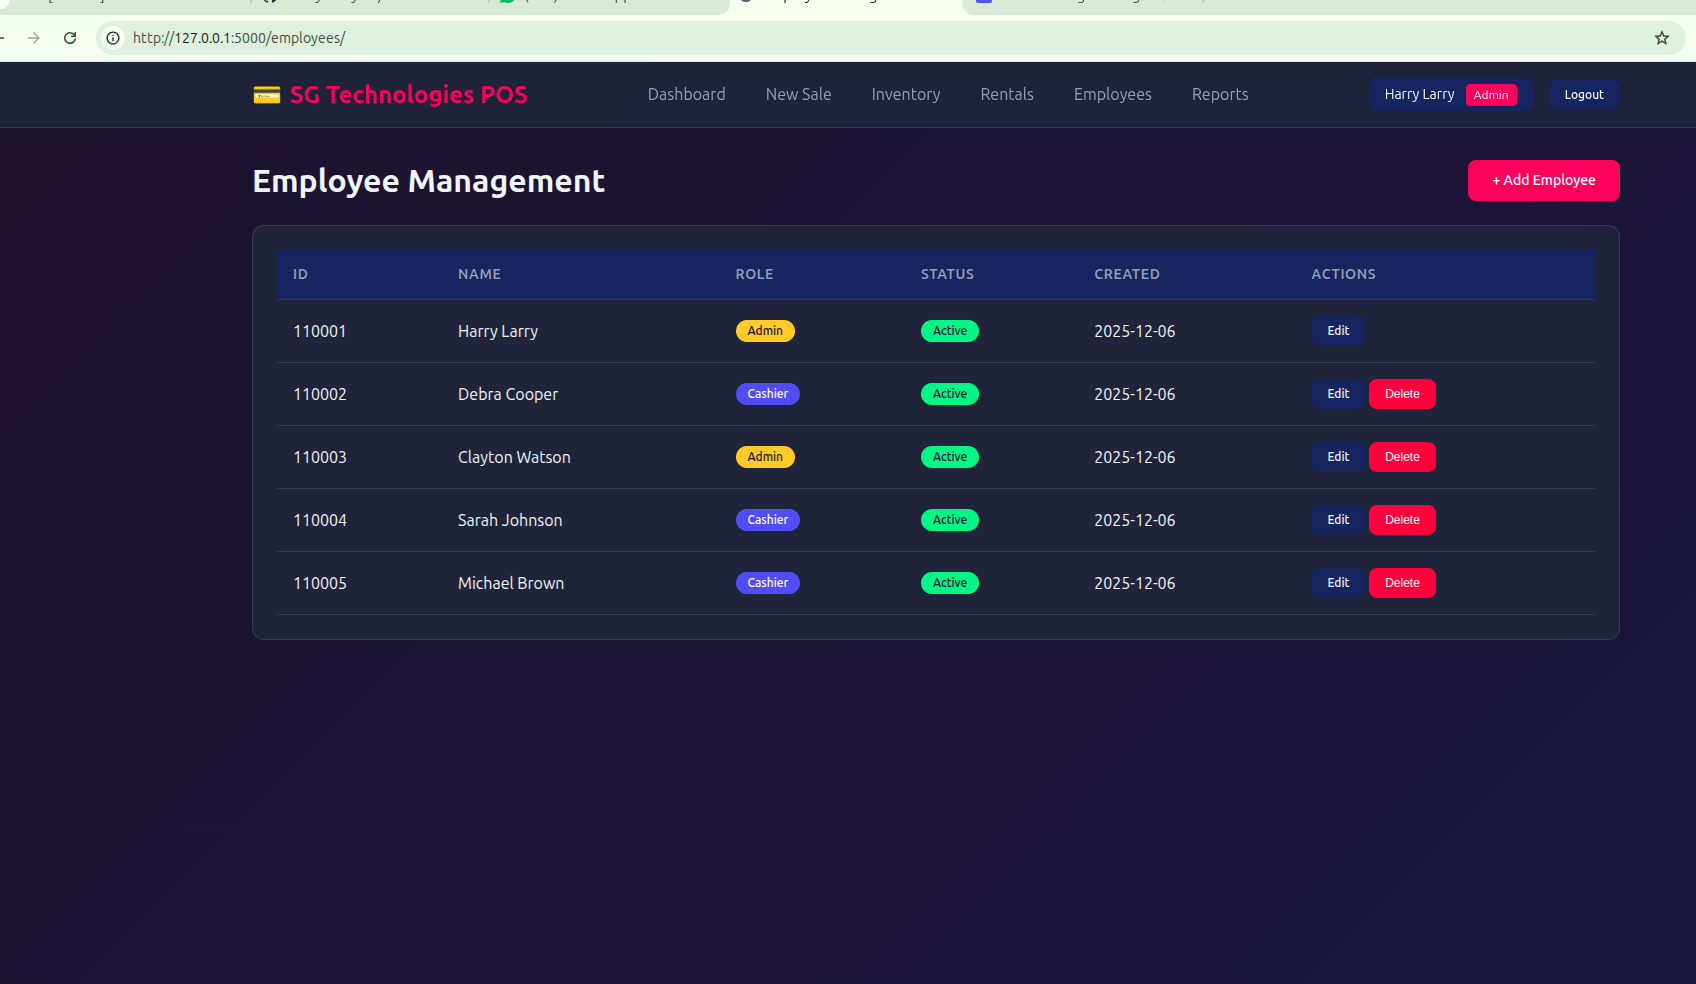
\includegraphics[width=0.95\textwidth]{images/6.png}
  \caption{Employee Management Interface -- Migrated employee data now includes
           unique IDs, role badges (Admin/Cashier), status indicators, creation
           timestamps, and action buttons. Passwords are securely hashed.}
  \label{fig:employee-management}
\end{figure}

\begin{figure}[h]
  \centering
  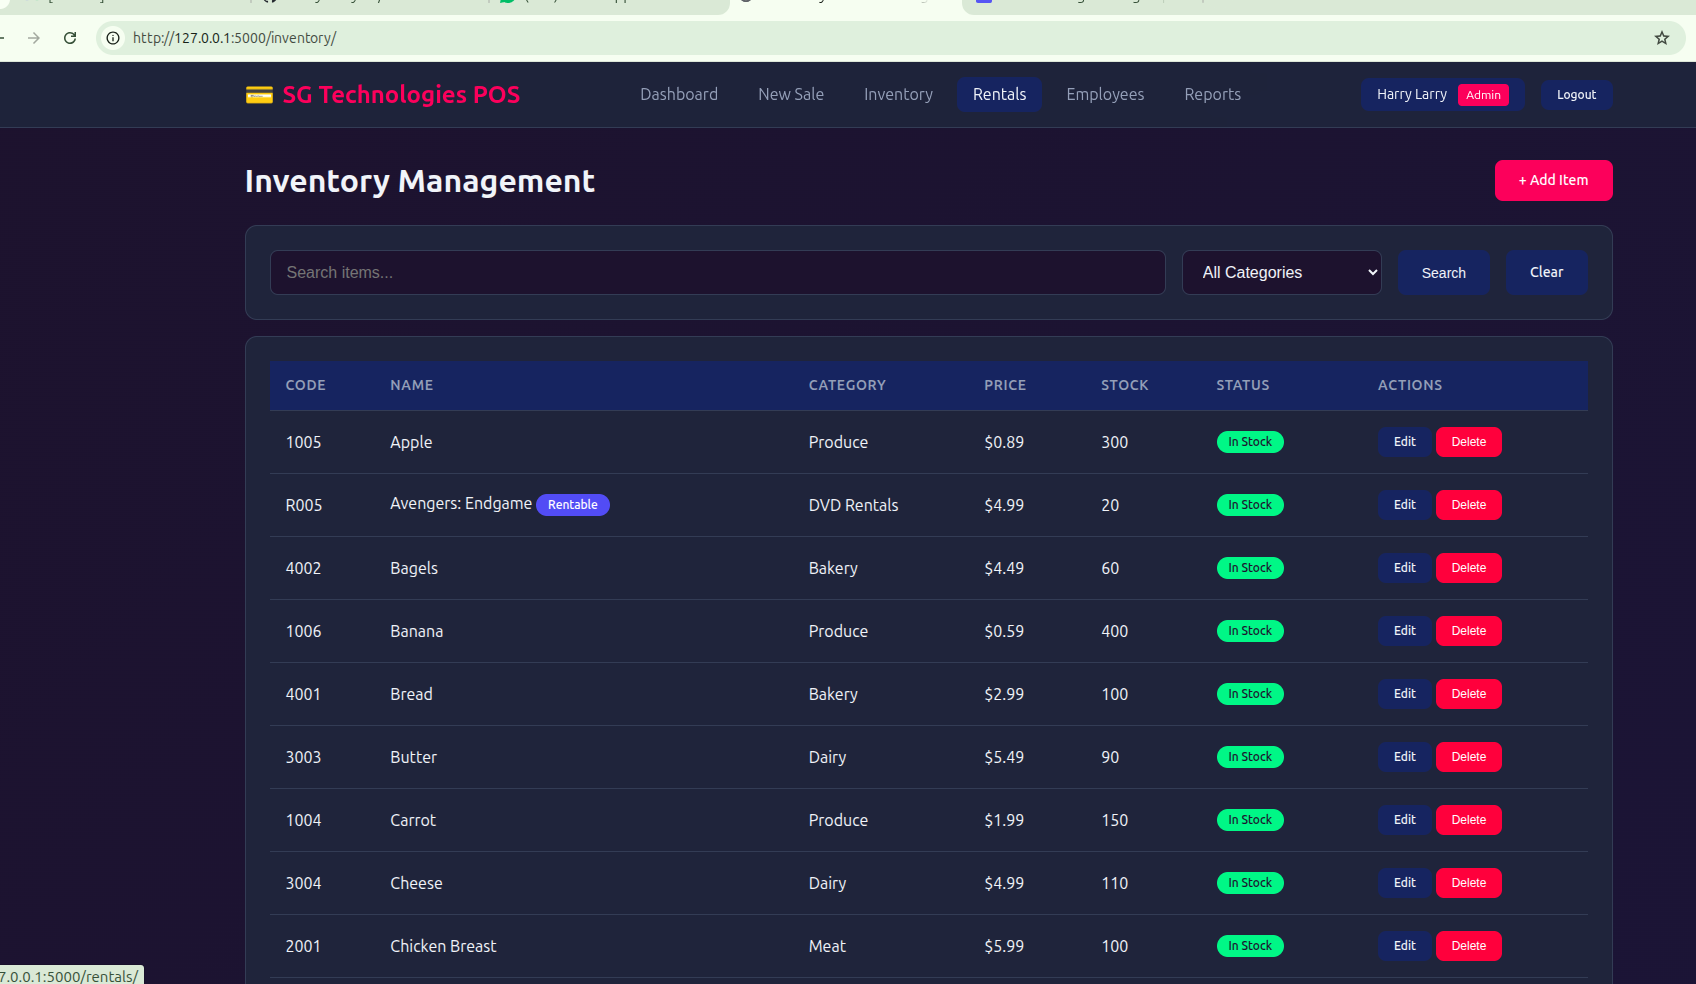
\includegraphics[width=0.95\textwidth]{images/3.png}
  \caption{Inventory Management Interface -- Migrated item data with proper
           categories (Produce, Bakery, Dairy, Meat, DVD Rentals), prices,
           stock quantities, status indicators, and the new ``Rentable'' badge
           for items that can be rented.}
  \label{fig:inventory-management}
\end{figure}

%=================================================
\chapter{Forward Engineering Report (Point 5)}
%=================================================

This chapter documents the forward engineering process for transforming
the legacy Java desktop POS system into a modern web-based application.

\section{Executive Summary}

Key achievements of the reengineered system:

\begin{itemize}[leftmargin=1.2cm]
  \item Transformed from a desktop Java Swing application to a
        web-based architecture.
  \item Migrated from legacy \texttt{.txt} files to a normalised
        SQLite/PostgreSQL database.
  \item Implemented secure password hashing instead of plain-text
        credentials.
  \item Introduced a proper layered architecture (MVC + Service Layer).
  \item Implemented comprehensive audit logging.
  \item Added a modern, responsive web UI.
  \item Achieved comprehensive automated test coverage on critical
        components.
\end{itemize}

\begin{figure}[h]
  \centering
  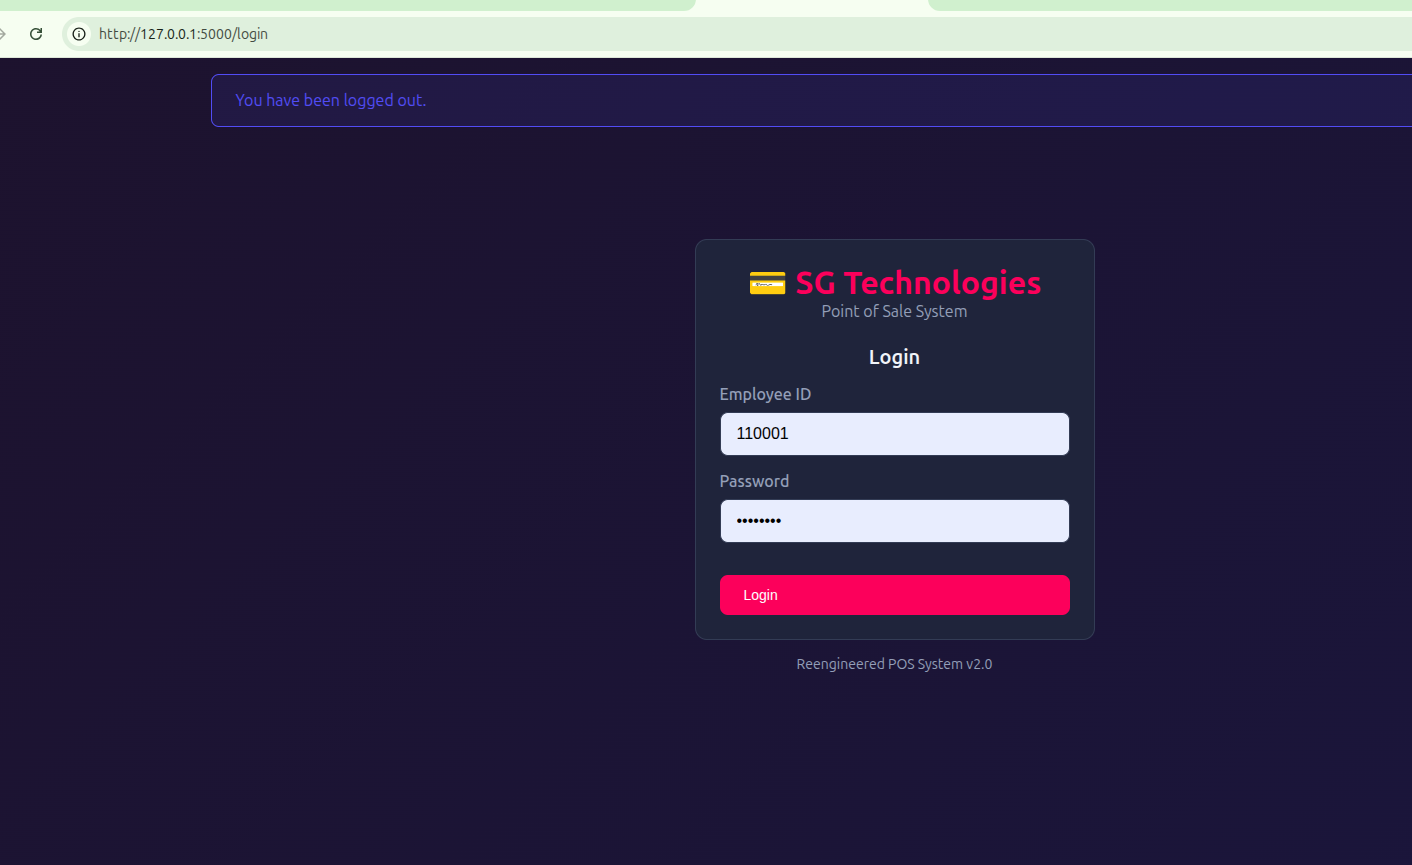
\includegraphics[width=0.85\textwidth]{images/1.png}
  \caption{Reengineered Login Interface -- Modern, responsive design with
           secure authentication. Employee ID and password are validated
           against the database with hashed password comparison.}
  \label{fig:login-interface}
\end{figure}

\section{Technology Stack Selection}

\subsection{Programming Language: Python 3.x}

Python was selected as the primary implementation language because of:

\begin{itemize}[leftmargin=1.2cm]
  \item Clean, readable syntax that improves maintainability.
  \item Rapid development cycle and rich ecosystem for web development.
  \item Large community support and extensive libraries.
\end{itemize}

\begin{table}[h]
  \centering
  \caption{Legacy vs Reengineered Language Choice}
  \begin{tabular}{p{3cm} p{4.5cm} p{4.5cm}}
    \toprule
    \textbf{Aspect} & \textbf{Legacy (Java)} & \textbf{Reengineered (Python)} \\
    \midrule
    Lines of Code & $\sim 2500$ & $\sim 1800$ \\
    Setup Time    & Complex (JDK, IDE, classpath) & Simple (\texttt{pip install}) \\
    Deployment    & JAR file                      & WSGI server \\
    Testing       & JUnit                         & Pytest (simpler, lightweight) \\
    \bottomrule
  \end{tabular}
\end{table}

\subsection{Web Framework: Flask}

Flask was chosen as the web framework due to:

\begin{itemize}[leftmargin=1.2cm]
  \item Lightweight core with minimal overhead.
  \item High flexibility, allowing architecture to be customised.
  \item Blueprint support for modular route organisation.
  \item Rich extension ecosystem (Flask-SQLAlchemy, Flask-Login, etc.).
\end{itemize}

\subsection{Database: SQLite / PostgreSQL}

\begin{table}[h]
  \centering
  \caption{Legacy Text Files vs Relational Database}
  \begin{tabular}{p{3cm} p{4.5cm} p{4.5cm}}
    \toprule
    \textbf{Feature} & \textbf{\texttt{.txt} Files} & \textbf{Relational DB} \\
    \midrule
    Data Integrity    & None                 & Constraints, types, keys \\
    Concurrent Access & File locks           & ACID transactions \\
    Query Capability  & Parse entire file    & SQL queries \\
    Relationships     & Embedded / duplicated & Foreign keys \\
    Scalability       & Poor                 & Excellent \\
    \bottomrule
  \end{tabular}
\end{table}

\section{Architecture Design}

\subsection{Layered Architecture + MVC}

\begin{figure}[h]
  \centering
  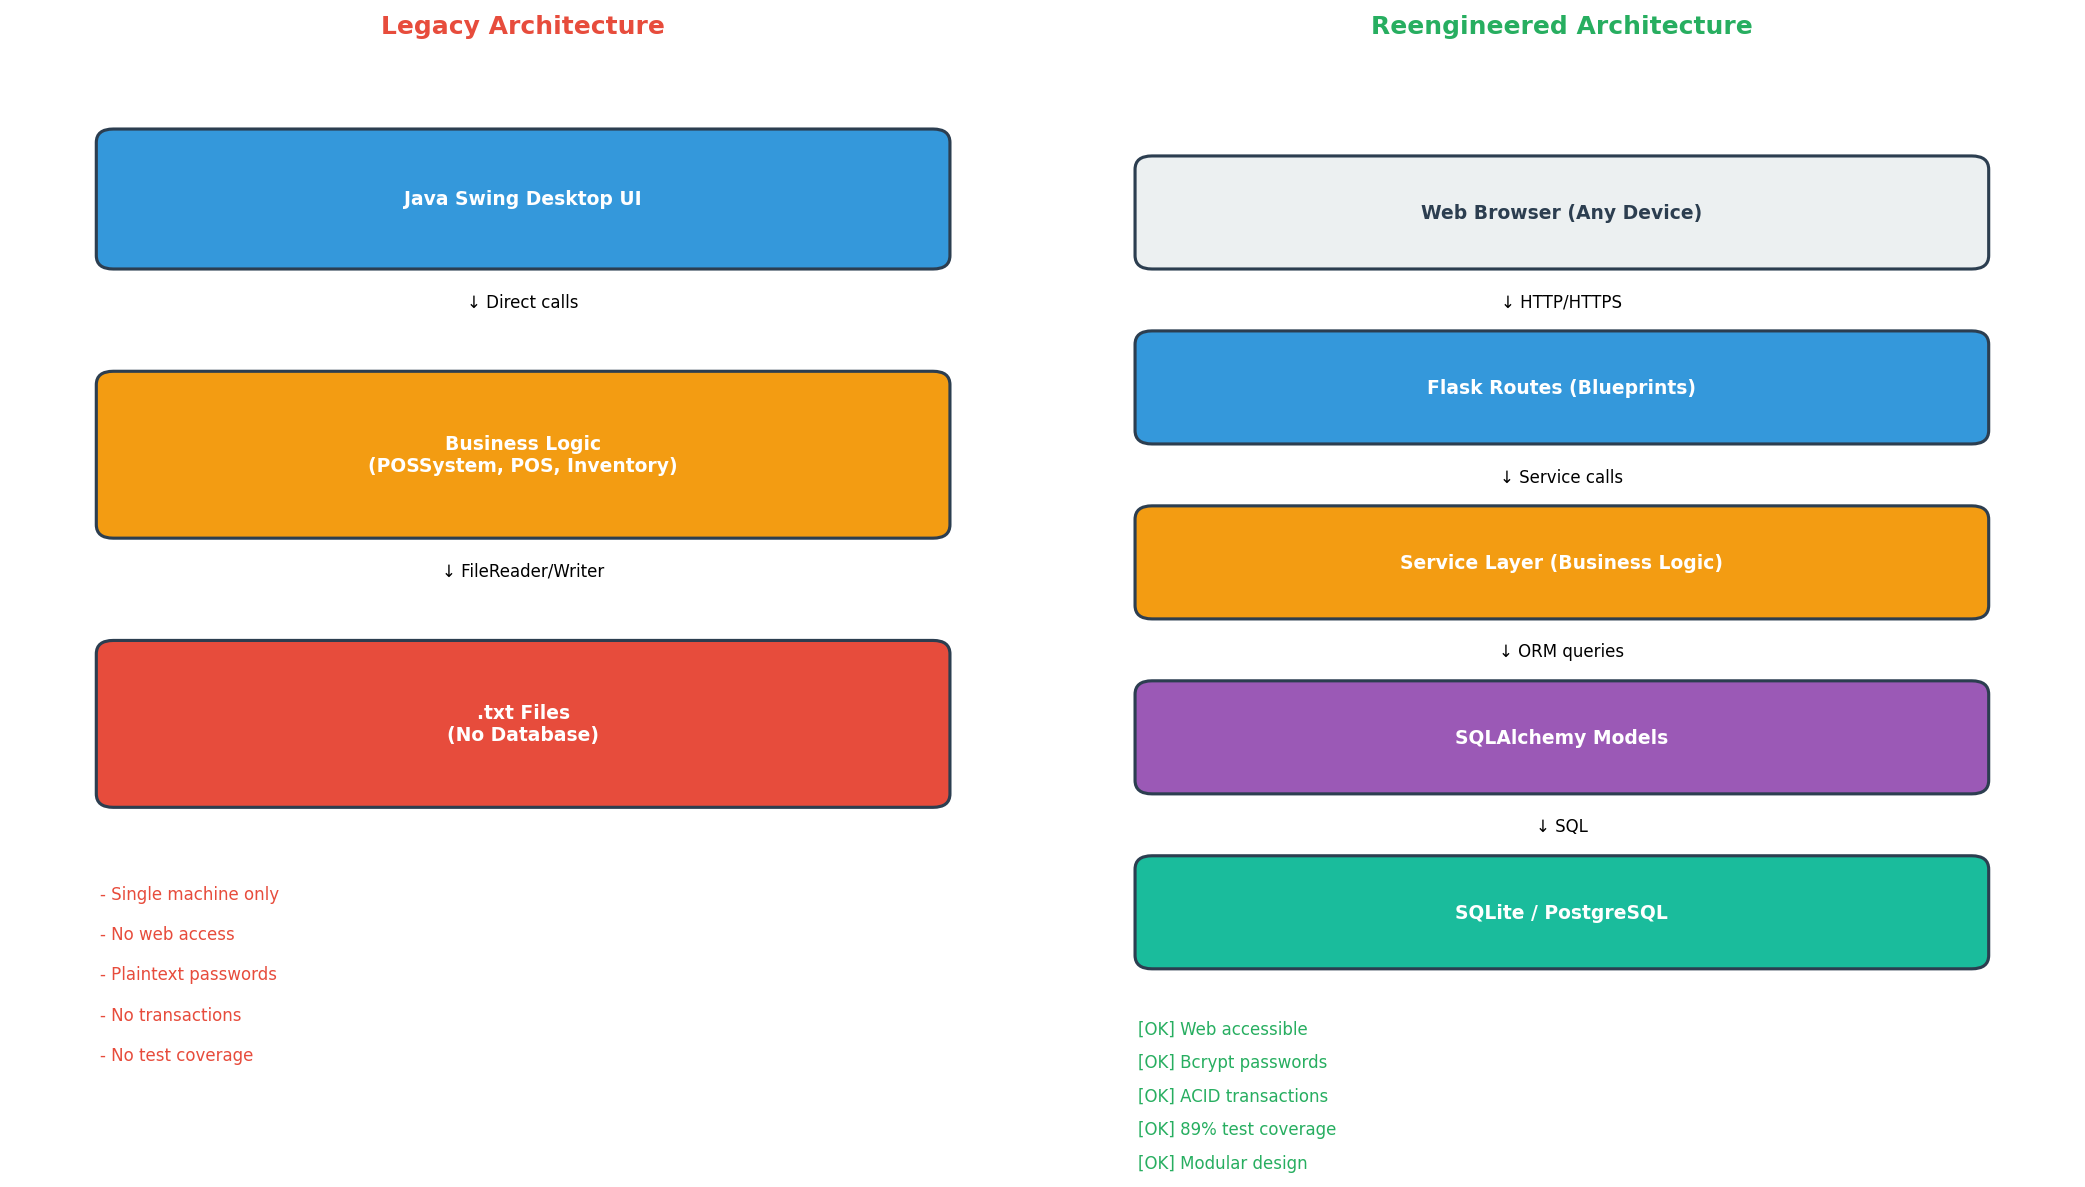
\includegraphics[width=0.95\textwidth]{images/architecture_comparison.png}
  \caption{Architecture Comparison -- Legacy monolithic Java Swing application (left)
           vs Reengineered layered Flask web application (right). The new architecture
           demonstrates clear separation of concerns with distinct Presentation,
           Business Logic, Data Access, and Database layers.}
  \label{fig:architecture-comparison}
\end{figure}

\begin{table}[h]
  \centering
  \caption{Architecture Layers}
  \begin{tabular}{p{3cm} p{4cm} p{5cm}}
    \toprule
    \textbf{Layer} & \textbf{Components} & \textbf{Responsibility} \\
    \midrule
    Presentation &
      Routes (Flask Blueprints), Templates (Jinja2), Static Assets &
      User interface and HTTP handling \\
    Business Logic &
      \texttt{AuthService}, \texttt{SalesService},
      \texttt{InventoryService}, \texttt{RentalService} &
      Core business rules \\
    Data Access &
      Models: \texttt{Employee}, \texttt{Item}, \texttt{Sale},
      \texttt{Rental}, \texttt{ActivityLog} &
      Database operations \\
    Database &
      SQLite / PostgreSQL &
      Data persistence \\
    \bottomrule
  \end{tabular}
\end{table}

\section{Design Patterns Used}

\begin{table}[h]
  \centering
  \caption{Design Patterns in the Reengineered System}
  \begin{tabular}{p{3cm} p{5cm} p{4cm}}
    \toprule
    \textbf{Pattern} & \textbf{Implementation} & \textbf{Benefit} \\
    \midrule
    MVC &
      Flask Blueprints + Jinja2 Templates + Models &
      Separation of concerns \\
    Repository &
      SQLAlchemy Models &
      Data access abstraction \\
    Service Layer &
      \texttt{app/services/} &
      Centralised business logic \\
    Factory &
      \texttt{create\_app()} in \texttt{\_\_init\_\_.py} &
      Configurable app creation \\
    Singleton &
      Flask extensions (\texttt{db}, \texttt{login\_manager}) &
      Single instance per app context \\
    Blueprint &
      Route modules under \texttt{app/routes/} &
      Modular code organisation \\
    \bottomrule
  \end{tabular}
\end{table}

\section{Component Mapping}

\begin{table}[h]
  \centering
  \caption{Legacy to Reengineered Component Mapping}
  \begin{tabular}{p{4cm} p{5cm} p{4cm}}
    \toprule
    \textbf{Legacy Component} & \textbf{Reengineered Component} & \textbf{Improvements} \\
    \midrule
    \texttt{Login\_Interface.java} &
      \texttt{routes/auth.py}, templates under \texttt{templates/auth/} &
      Session-based auth, secure passwords \\
    \texttt{Employee.java} &
      \texttt{models/employee.py} &
      Password hashing, relationships \\
    \texttt{Item.java} &
      \texttt{models/item.py} &
      Stock tracking, categories \\
    \texttt{POS.java} &
      \texttt{services/sales\_service.py} &
      Transaction management \\
    \texttt{.txt} files &
      SQLite/PostgreSQL &
      ACID-compliant persistence \\
    \bottomrule
  \end{tabular}
\end{table}

\section{User Interface Screenshots}

The following screenshots demonstrate the reengineered system's modern web interface,
showcasing the implementation of all major functional areas.

\subsection{Role-Based Dashboards}

\begin{figure}[h]
  \centering
  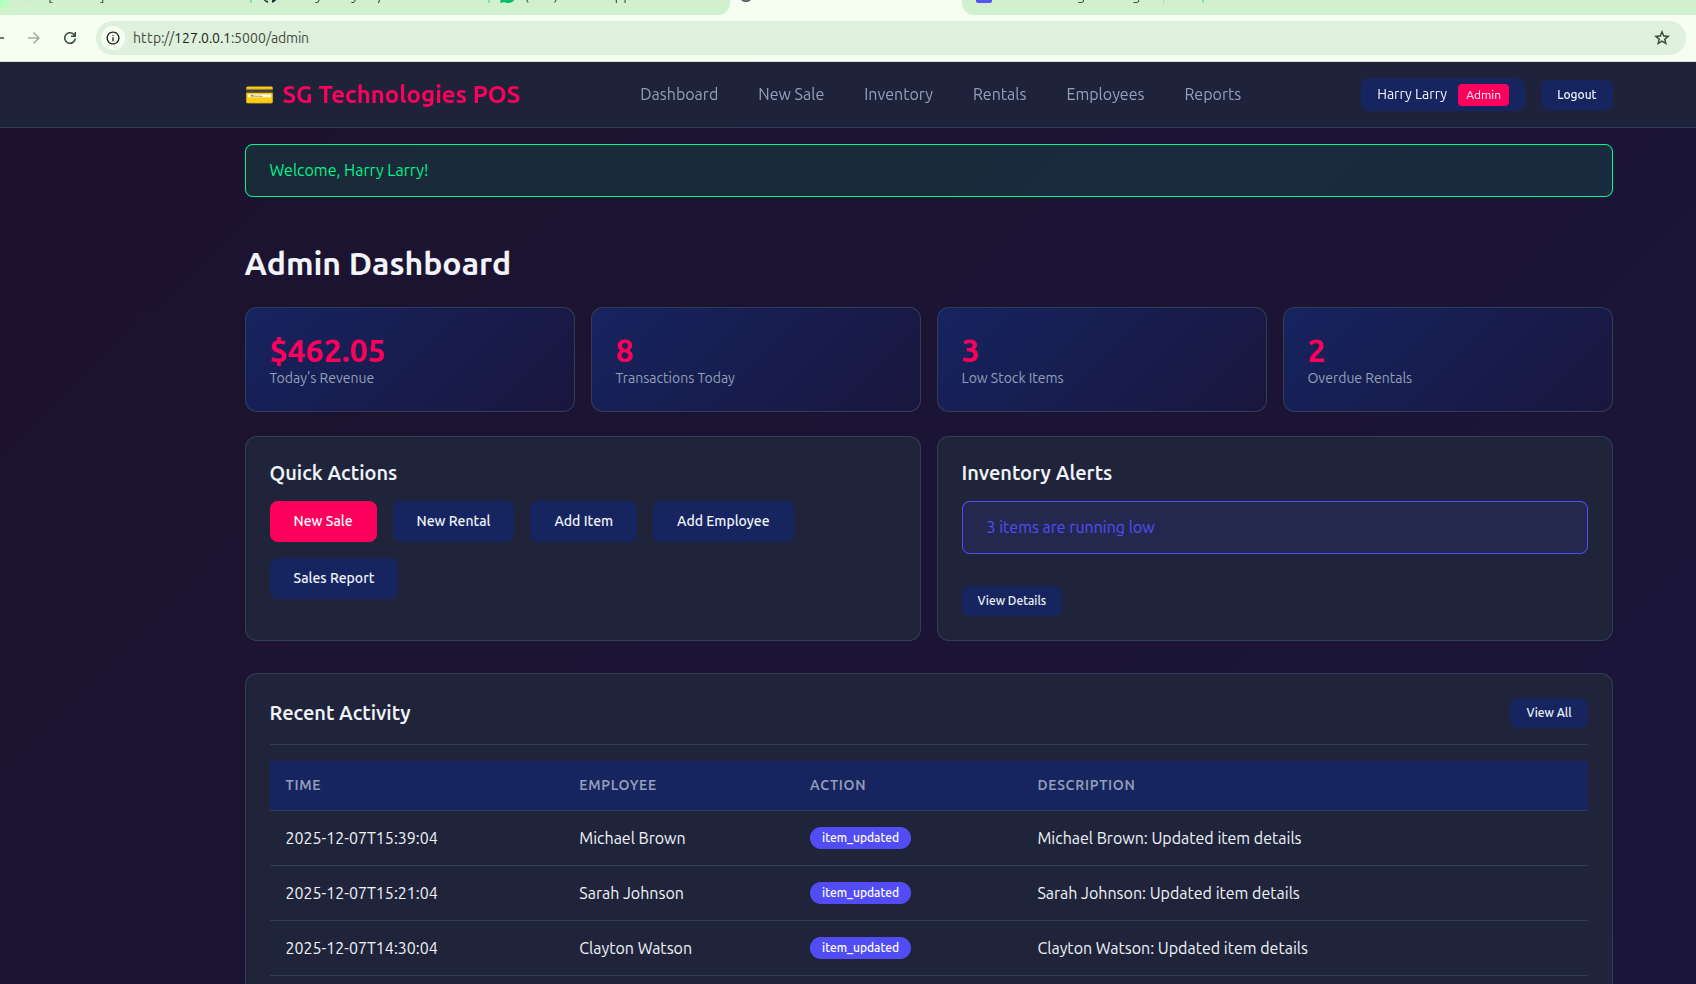
\includegraphics[width=0.95\textwidth]{images/2.png}
  \caption{Admin Dashboard -- Displays today's revenue (\$462.05), transaction count,
           low stock items (3), and overdue rentals (2). Quick actions allow admins
           to create sales, rentals, add items, and add employees. Recent activity
           log shows audit trail of all system actions.}
  \label{fig:admin-dashboard}
\end{figure}

\begin{figure}[h]
  \centering
  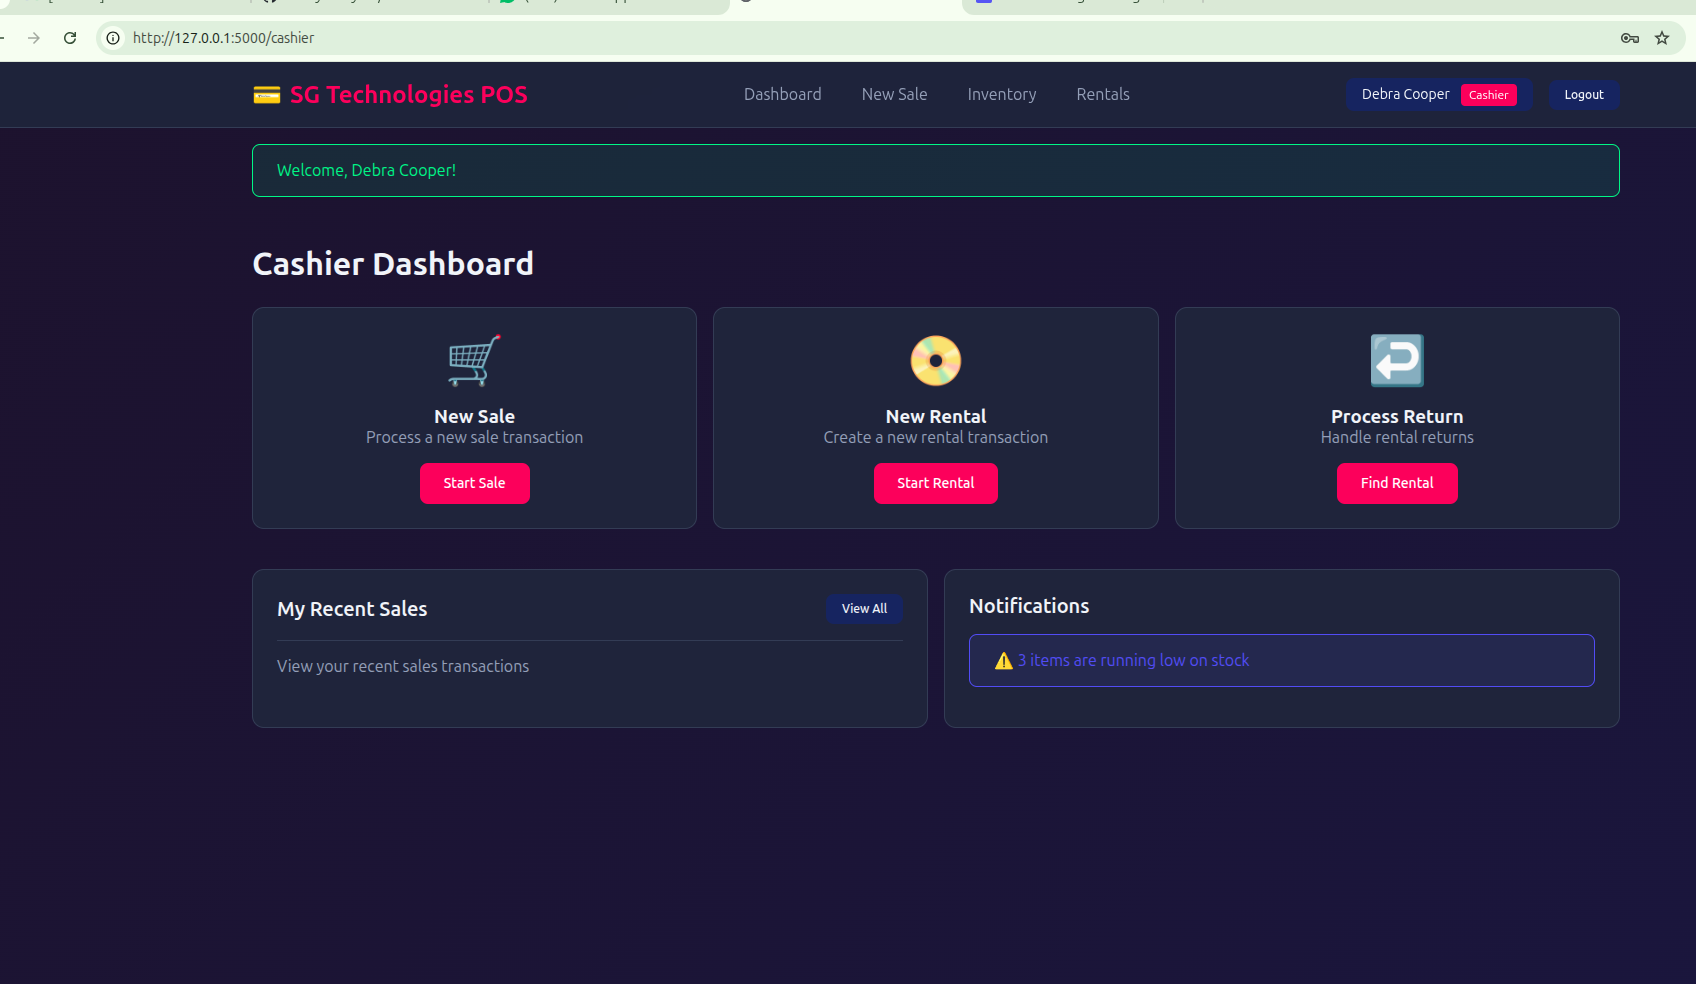
\includegraphics[width=0.95\textwidth]{images/7.png}
  \caption{Cashier Dashboard -- Simplified interface for cashier role with quick
           access to New Sale, New Rental, and Process Return functions. Shows
           notifications for low stock items and recent sales history.}
  \label{fig:cashier-dashboard}
\end{figure}

\subsection{Point of Sale Interface}

\begin{figure}[h]
  \centering
  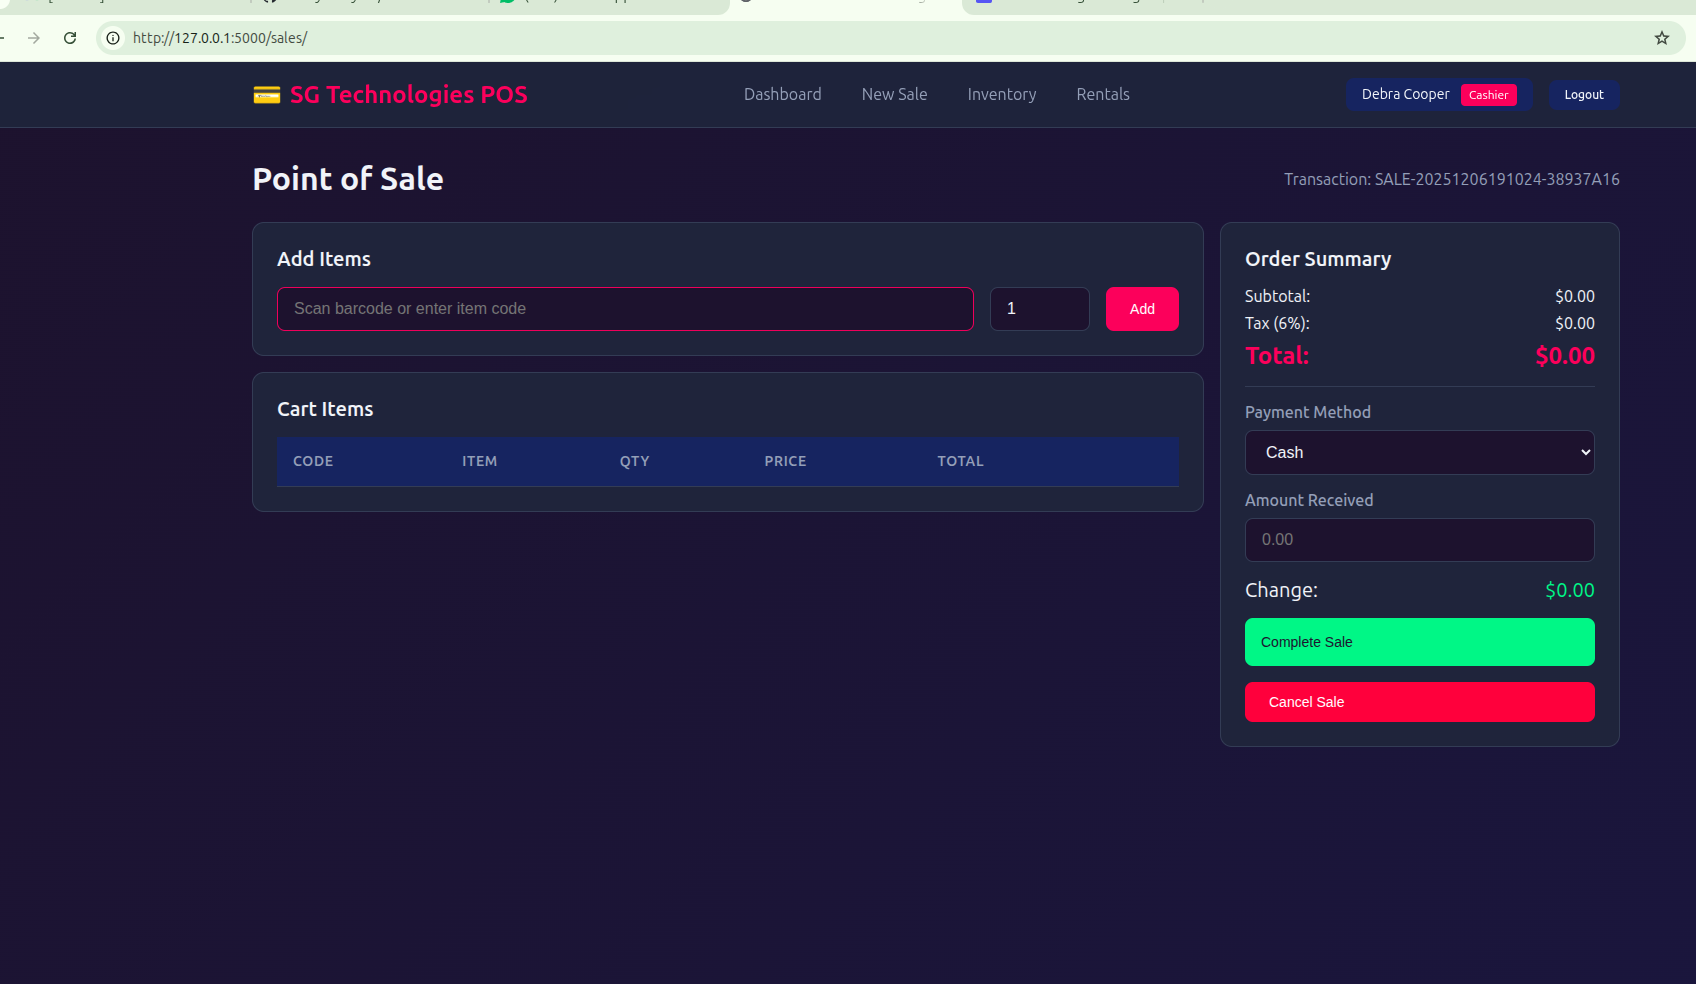
\includegraphics[width=0.95\textwidth]{images/8.png}
  \caption{Point of Sale Interface -- Modern cart-based sales system with barcode/item
           code entry, real-time order summary showing subtotal, tax (6\%), and total.
           Payment method selection (Cash) with change calculation and Complete/Cancel
           buttons.}
  \label{fig:pos-interface}
\end{figure}

\subsection{Rental Management}

\begin{figure}[h]
  \centering
  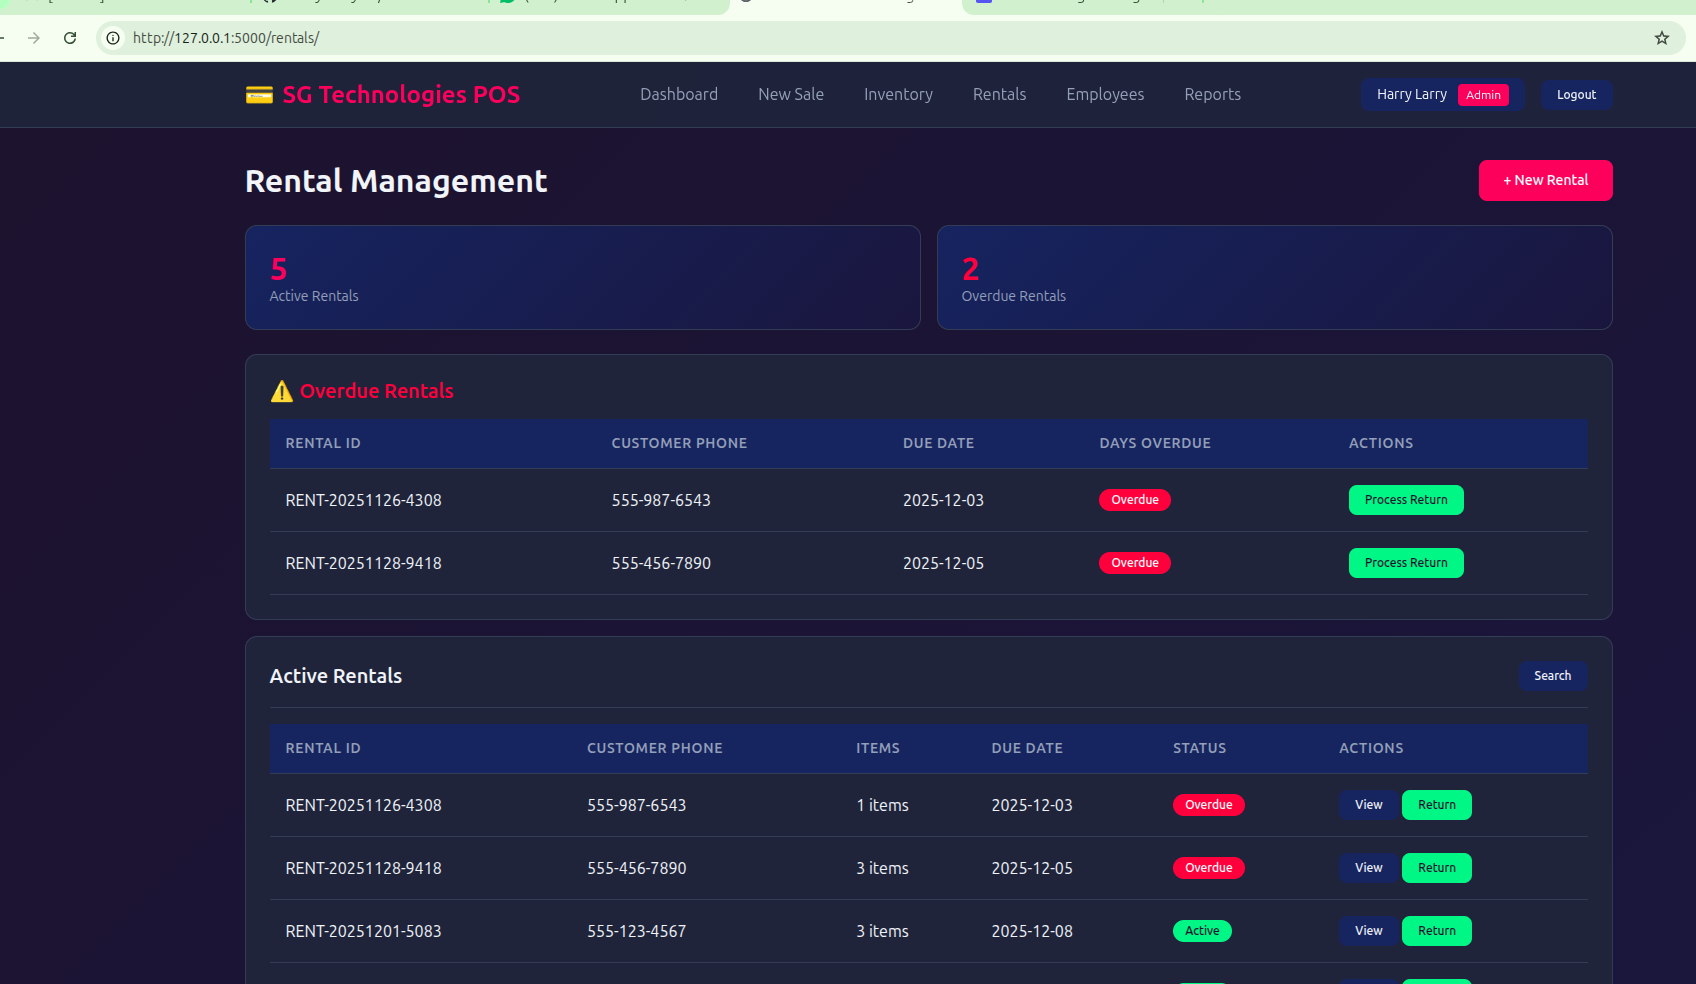
\includegraphics[width=0.95\textwidth]{images/4.png}
  \caption{Rental Management Interface -- Shows active rentals (5) and overdue rentals
           (2) with customer phone, due dates, and status indicators. Includes ``Process
           Return'' and ``View'' actions for each rental transaction.}
  \label{fig:rental-management}
\end{figure}

\subsection{Reports Dashboard}

\begin{figure}[h]
  \centering
  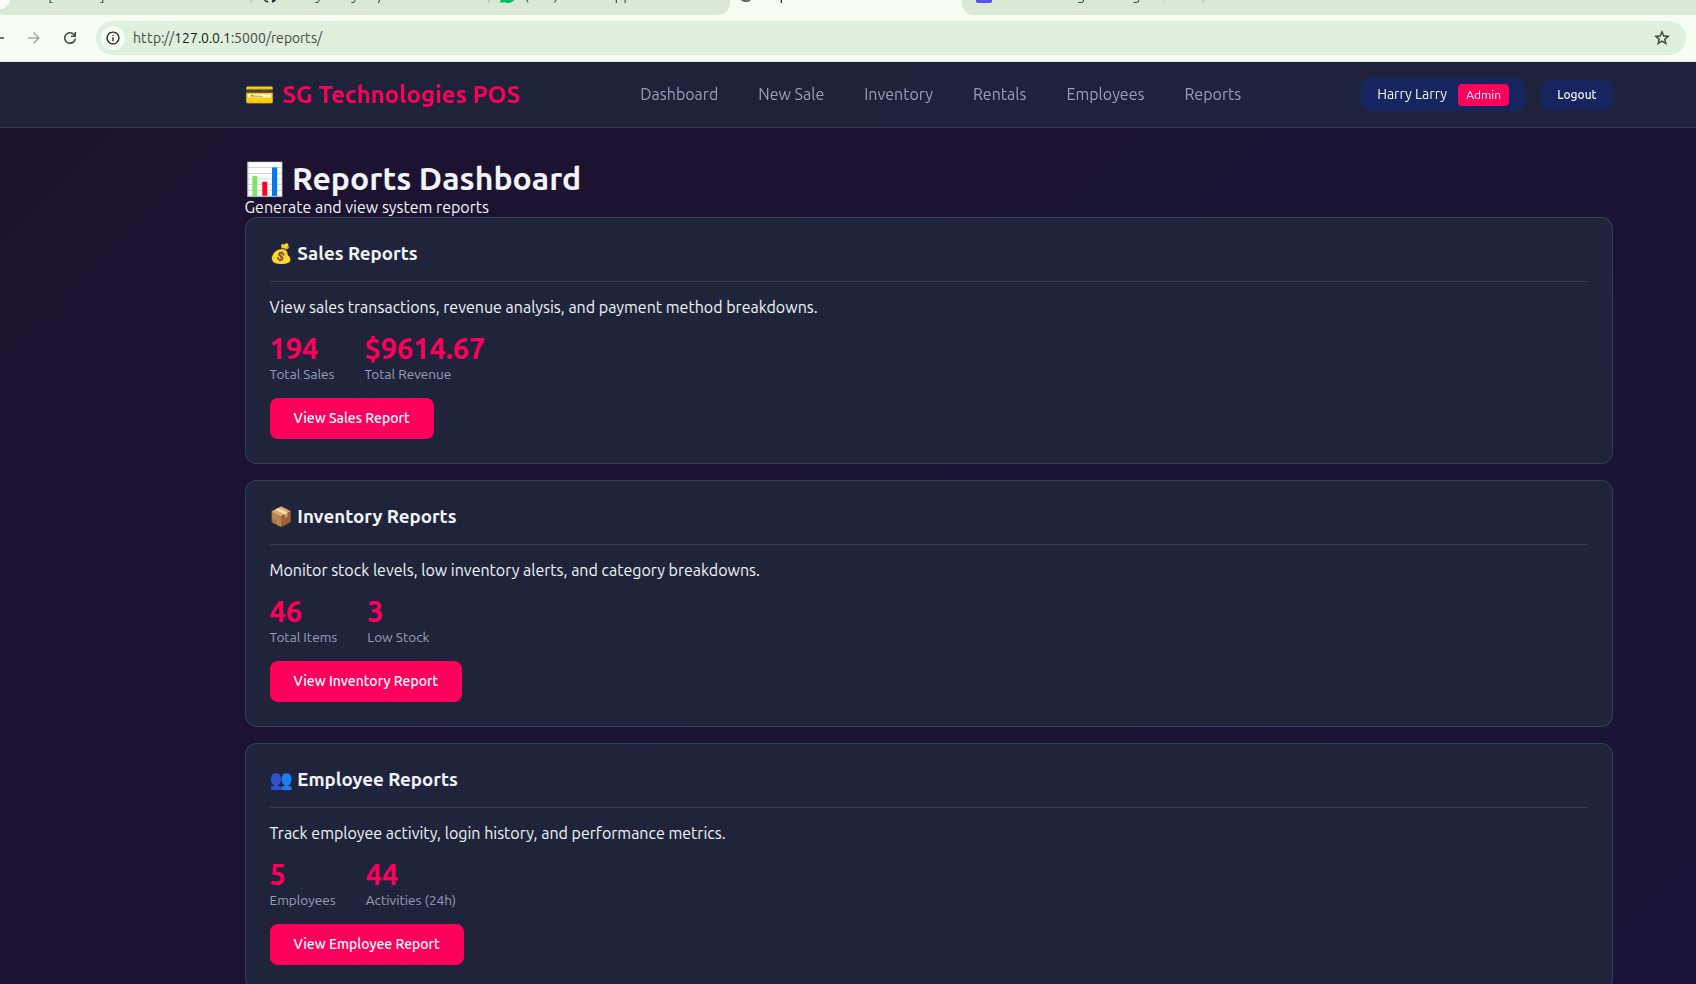
\includegraphics[width=0.95\textwidth]{images/5.png}
  \caption{Reports Dashboard -- Comprehensive reporting with Sales Reports (194 total
           sales, \$9614.67 revenue), Inventory Reports (46 items, 3 low stock), and
           Employee Reports (5 employees, 44 activities in 24h).}
  \label{fig:reports-dashboard}
\end{figure}

\section{Deployment Guide}

\subsection{Development Setup}

\begin{enumerate}[leftmargin=1.2cm]
  \item Navigate to reengineered directory: \texttt{cd reengineered}
  \item Create virtual environment: \texttt{python -m venv venv}
  \item Activate virtual environment: \texttt{source venv/bin/activate}
  \item Install dependencies: \texttt{pip install -r requirements.txt}
  \item Run development server: \texttt{python run.py}
  \item Access the app at \url{http://127.0.0.1:5000}
\end{enumerate}

\subsubsection*{Default Login Credentials}

\begin{itemize}[leftmargin=1.2cm]
  \item Admin: \texttt{110001 / admin123}
  \item Cashier: \texttt{110002 / cashier123}
\end{itemize}

%=================================================
\chapter{Reengineering Plan and Migration (Point 6)}
%=================================================

\section{Objectives}

The goal of this reengineering plan is to transform the legacy Java desktop--based
Point-of-Sale (POS) system, which relies on plain text (\texttt{.txt}) files for
persistence, into a modern, web-based architecture with a normalized relational
database backend.

This plan covers:
\begin{itemize}
  \item The phased reengineering approach from inventory analysis to forward engineering.
  \item A realistic timeline with milestones and responsibilities.
  \item The end-to-end data migration strategy from text files to a relational database.
  \item Risk-aware execution, aligned with the risk analysis and testing strategy.
\end{itemize}

\section{Reengineering Process Flow}

Figure~\ref{fig:reengineering-flow} illustrates the complete reengineering
process from legacy system analysis to the delivery of the modernized web
application.

\begin{figure}[h]
  \centering
  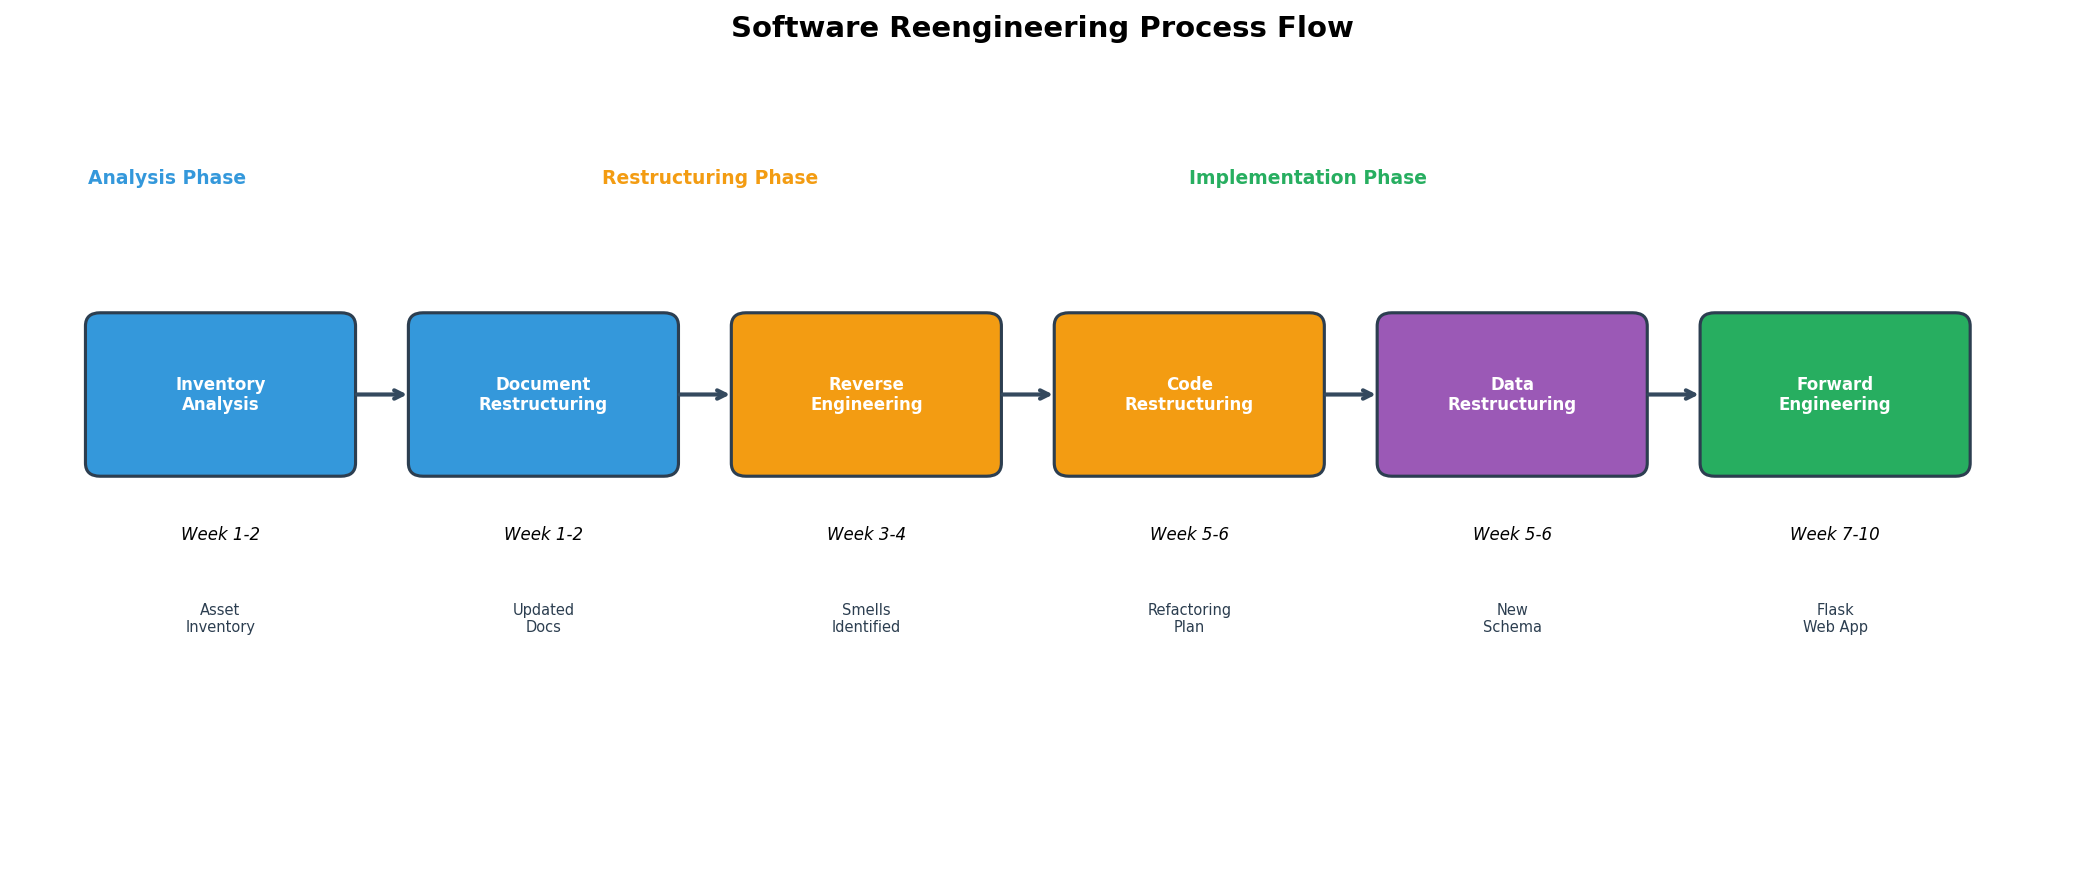
\includegraphics[width=0.95\textwidth]{images/reengineering_flow.png}
  \caption{Software Reengineering Process Flow -- The systematic transformation
           from legacy Java desktop POS system to modern Flask web application,
           following all phases of the reengineering model.}
  \label{fig:reengineering-flow}
\end{figure}

\section{Phase Overview}

\begin{table}[h]
  \centering
  \caption{Reengineering Phases Overview}
  \begin{tabular}{p{3.2cm} p{10.0cm}}
    \toprule
    \textbf{Phase} & \textbf{Description} \\
    \midrule
    Inventory Analysis &
      Identify and classify all legacy assets (Java source files, libraries,
      configuration files, and text-based ``database'' files). \\
    Document Restructuring &
      Reconstruct and reorganize technical documentation to reflect the actual
      structure, modules, and data flows. \\
    Reverse Engineering &
      Analyze the legacy codebase to recover design, workflows, and data
      structures. Identify code smells and data smells. \\
    Code Restructuring &
      Propose and apply refactorings to improve modularity, readability,
      and separation of concerns. \\
    Data Restructuring &
      Redesign the data model as a normalized relational schema (3NF),
      define table structures and constraints. \\
    Forward Engineering &
      Implement the reengineered POS system as a web-based application. \\
    \bottomrule
  \end{tabular}
\end{table}

\section{Timeline and Milestones}

\begin{table}[h]
  \centering
  \caption{High-Level Reengineering Timeline}
  \begin{tabular}{p{2.2cm} p{10.0cm}}
    \toprule
    \textbf{Weeks} & \textbf{Planned Activities and Milestones} \\
    \midrule
    Week 1--2 &
      \textbf{Inventory Analysis \& Document Restructuring} --
      Collect all legacy artefacts, build asset inventory and dependency map. \\
    Week 3--4 &
      \textbf{Reverse Engineering \& Smell Detection} --
      Recover workflows, identify code and data smells. \\
    Week 5--6 &
      \textbf{Code Restructuring \& Data Restructuring Design} --
      Define repository and service abstractions, design normalized schema. \\
    Week 7--8 &
      \textbf{Forward Engineering (Web Architecture)} --
      Implement Flask application structure (models, services, routes). \\
    Week 9 &
      \textbf{Data Migration Implementation \& Dry Runs} --
      Implement migration script, execute dry runs, verify record counts. \\
    Week 10 &
      \textbf{Testing, Risk Mitigation \& Finalization} --
      Execute automated tests, validate risk mitigations, complete documentation. \\
    \bottomrule
  \end{tabular}
\end{table}

\section{Risk Considerations}

The reengineering plan explicitly addresses potential risks at each phase.
Table~\ref{tab:phase-risks} summarizes the key risks and their mitigation
strategies integrated into the timeline.

\begin{table}[h]
  \centering
  \caption{Risk Considerations by Phase}
  \label{tab:phase-risks}
  \begin{tabular}{p{3.5cm} p{4.5cm} p{5cm}}
    \toprule
    \textbf{Phase} & \textbf{Key Risk} & \textbf{Mitigation Strategy} \\
    \midrule
    Inventory Analysis &
      Incomplete asset identification &
      Systematic directory scan; cross-reference with documentation \\
    Reverse Engineering &
      Misunderstanding legacy workflows &
      Trace execution paths; validate with sample transactions \\
    Code Restructuring &
      Breaking existing functionality &
      Incremental refactoring; regression testing after each change \\
    Data Restructuring &
      Data loss during schema migration &
      Full backup before migration; staged migration with validation \\
    Forward Engineering &
      Architecture drift from design &
      Code reviews; adherence to layered architecture patterns \\
    Migration Execution &
      Production data corruption &
      Dry runs on test data; rollback scripts prepared \\
    \bottomrule
  \end{tabular}
\end{table}

\subsection{Critical Risk Mitigation}

The following high-priority risks are addressed throughout the plan:

\begin{itemize}
  \item \textbf{R1 -- Data Loss:} Mandatory backup of all \texttt{.txt} files before
        any migration; record count verification at each stage.
  \item \textbf{R2 -- Authentication Security:} Passwords are hashed during the
        Transform phase; plaintext passwords are never stored in the new database.
  \item \textbf{R3 -- Functional Regression:} All original POS functionality
        (sales, rentals, returns, inventory) is verified through automated tests
        before deployment.
  \item \textbf{R4 -- Timeline Overrun:} Buffer time allocated in Weeks 9--10 for
        unexpected issues; phased approach allows for incremental delivery.
\end{itemize}

\section{Migration Strategy}

\subsection{Migration Objectives}

\begin{itemize}
  \item Preserve \textbf{100\%} of valid legacy data from text files.
  \item Eliminate structural, security, and quality smells via normalization.
  \item Ensure that migration is \emph{idempotent} and \emph{verifiable}
        through record counts and integrity checks.
\end{itemize}

\subsection{Migration Phases}

\begin{table}[h]
  \centering
  \caption{Data Migration Phases}
  \begin{tabular}{p{3.0cm} p{9.7cm}}
    \toprule
    \textbf{Phase} & \textbf{Description} \\
    \midrule
    Backup &
      Copy all legacy \texttt{Database/} files to a timestamped backup folder. \\
    Parse &
      Read and parse legacy text files, converting each line into structured
      in-memory objects. \\
    Transform &
      Map parsed records to the new relational schema: normalize repeated groups,
      convert date formats, hash passwords. \\
    Validate &
      Perform integrity checks before committing: verify counts, ensure no
      missing mandatory fields. \\
    Load &
      Insert transformed data into the database using SQLAlchemy models. \\
    Verify &
      Run post-migration verification queries: compare record counts, check for
      orphan records. \\
    \bottomrule
  \end{tabular}
\end{table}

\section{Roles and Responsibilities}

\begin{table}[h]
  \centering
  \caption{Roles and Responsibilities Across Phases}
  \begin{tabular}{p{4.5cm} p{3.2cm} p{5.0cm}}
    \toprule
    \textbf{Member} & \textbf{Primary Phases} & \textbf{Key Responsibilities} \\
    \midrule
    Abdul Faheem (22i--2629) &
      Inventory, Reverse Engineering &
      Asset inventory and dependency mapping; legacy workflow analysis;
      identification of code/data smells; initial legacy documentation. \\
    Sheryar Ali (22i--2623) &
      Code Restructuring, Data Restructuring &
      Refactoring proposals; design of the normalized relational schema;
      specification of migration rules and mapping. \\
    Husnain Akram (22i--2464) &
      Forward Engineering, Testing, Migration &
      Implementation of the Flask-based web architecture; migration scripts;
      automated tests and risk mitigation activities. \\
    \bottomrule
  \end{tabular}
\end{table}

\section{Deliverables and Exit Criteria}

The reengineering and migration effort is considered complete when:

\begin{itemize}
  \item The normalized relational schema is implemented and documented.
  \item All relevant legacy data has been successfully migrated with
        verified record counts and integrity checks.
  \item The Flask-based POS application supports the original functional
        requirements (sales, rentals, inventory, employee management).
  \item Automated tests (models, services, routes) pass with the targeted
        coverage level and are repeatable via the project test suite.
  \item Risk mitigations for data loss, authentication, SQL injection,
        and concurrency are in place and documented.
  \item Dual documentation (legacy vs reengineered) and the signed
        work-distribution table are finalized.
\end{itemize}
